\chapter{Sprint 3 - Design and implementation}

\section*{Introduction}
\addcontentsline{toc}{section}{Introduction}
In Sprint 3, administrators focused on improving rental order reporting by adding dynamic filters. 
\section{Sprint 3 Backlog}
Table \ref{tab:sprint3_backlog} lists the planned tasks for this sprint.

\begin{longtable}{|c|p{8cm}|c|}
    \hline
    \rowcolor{purple!20} \textbf{N°} & \textbf{Tasks} & \textbf{Duration} \\ \hline
    \endfirsthead
    \hline
    \rowcolor{purple!20} \textbf{N°} & \textbf{Tasks} & \textbf{Duration} \\ \hline
    \endhead
    1 & As an administrator, I can generate rental order reports. & 3 Day \\ \hline
    2 & As an administrator, I can view rental reports in different chart formats (bar, pie, line, pivot). & 3 Day \\ \hline
    3 & As an administrator, I can filter rental reports by measure (order date, customer, product). & 2 Days \\ \hline
    4 & As an administrator, I can adjust report view modes and filters dynamically. & 2 Days \\ \hline
    \caption{Sprint 3 Backlog for Rental Order Reporting}
    \label{tab:sprint3_backlog}
\end{longtable}

\section{Functional Specifications}

\subsection{Use Case Diagram}
This section presents the functional specifications for the Rental Order Reporting module. Figure \ref{fig:sprint3_use_case_diagram} depicts the use case diagram that outlines the interactions and functionalities within this module.

\begin{figure}[h]
    \centering
    \makebox[\textwidth][c]{%
        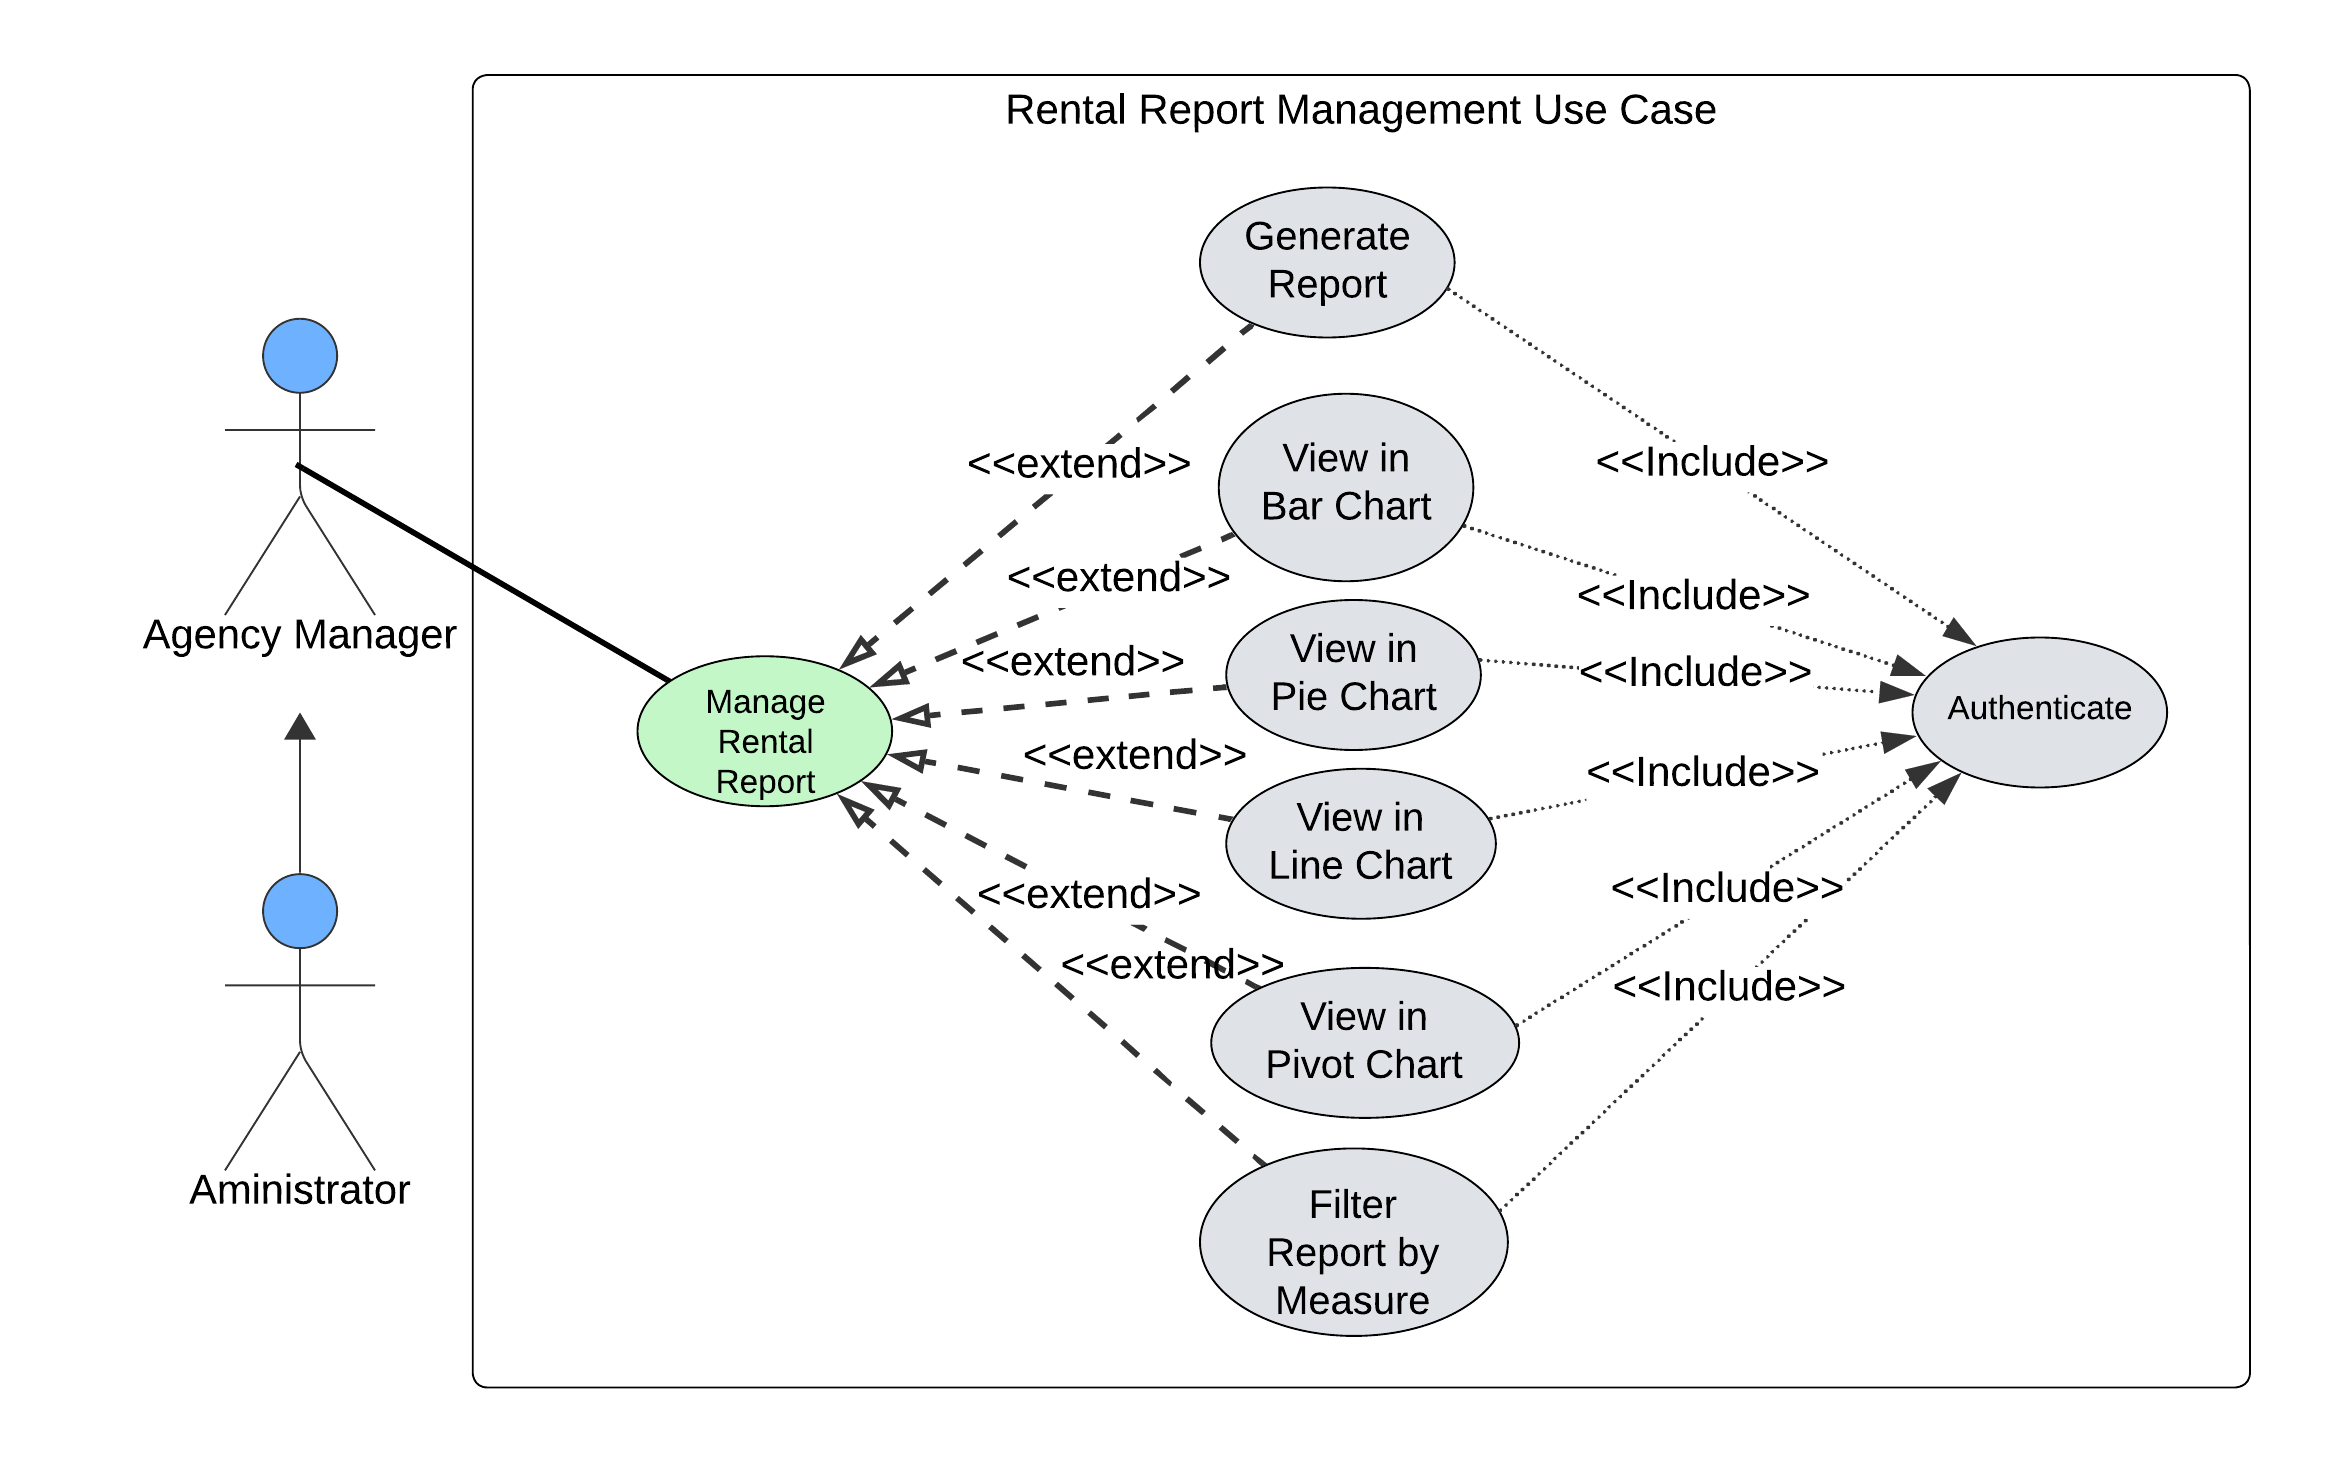
\includegraphics[width=1.2\textwidth]{sprint3/sprint3usecase.png}} % replace with your image path
    \caption{Sprint 3 Use Case Diagram}
    \label{fig:sprint3_use_case_diagram}
\end{figure}

\subsection{Report Management Sequence Diagram}
The sequence diagram below illustrates the process of generating rental order reports:

\begin{itemize}
    \item Administrator selects report generation.
    \item System shows report configuration form.
    \item Administrator picks view mode (bar, pie, line, pivot).
    \item Applies filters (order date, customer, product), generates and displays report, and adjusts as needed.
\end{itemize}
Figure \ref{fig:report_sequence_diagram} illustrates the sequence diagram for the process of generating rental order reports in Sprint 3.

\begin{figure}[h]
    \centering
    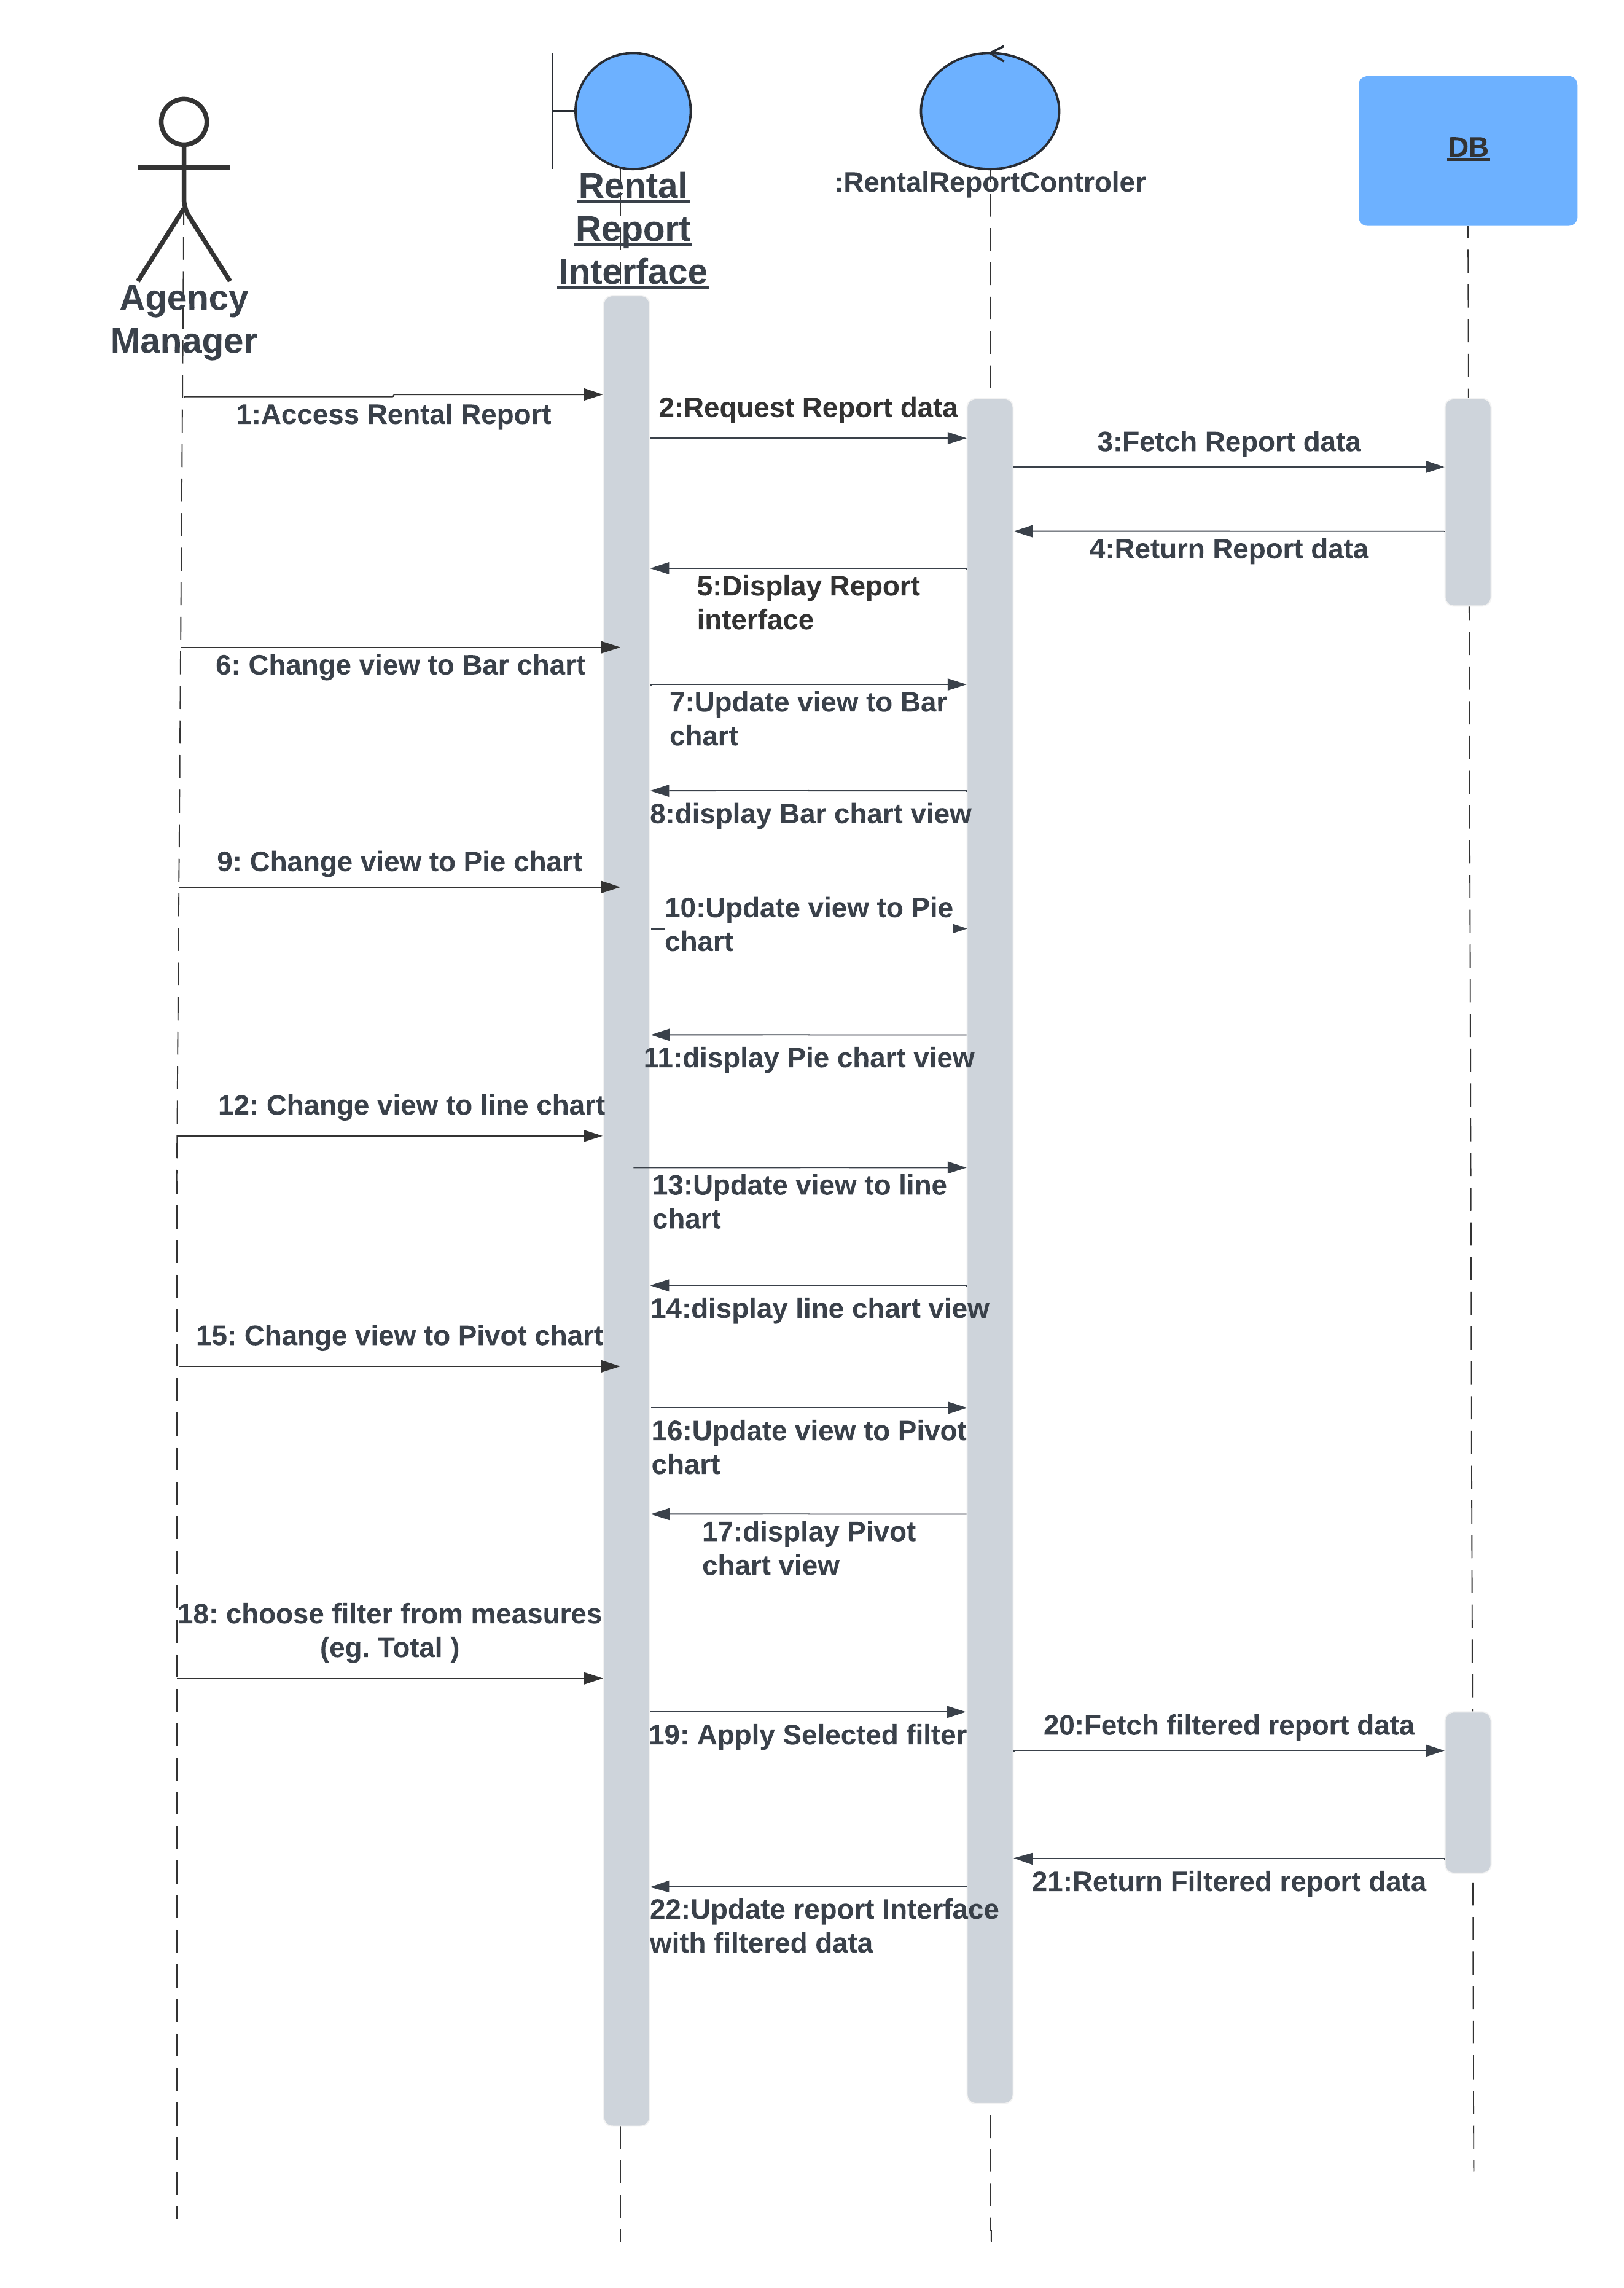
\includegraphics[width=0.7\textwidth]{sprint3/Sprint3Sequence.png} % replace with your image path
    \caption{Sequence Diagram for "Generating Rental Order Reports"}
    \label{fig:report_sequence_diagram}
\end{figure}


\section{Sprint Realization}


\subsection{Bar Chart View}
Figure \ref{fig:bar_chart_view} shows the rental order report in a bar chart format. This view helps in comparing rental orders over different periods.

\begin{figure}[h]
    \centering
    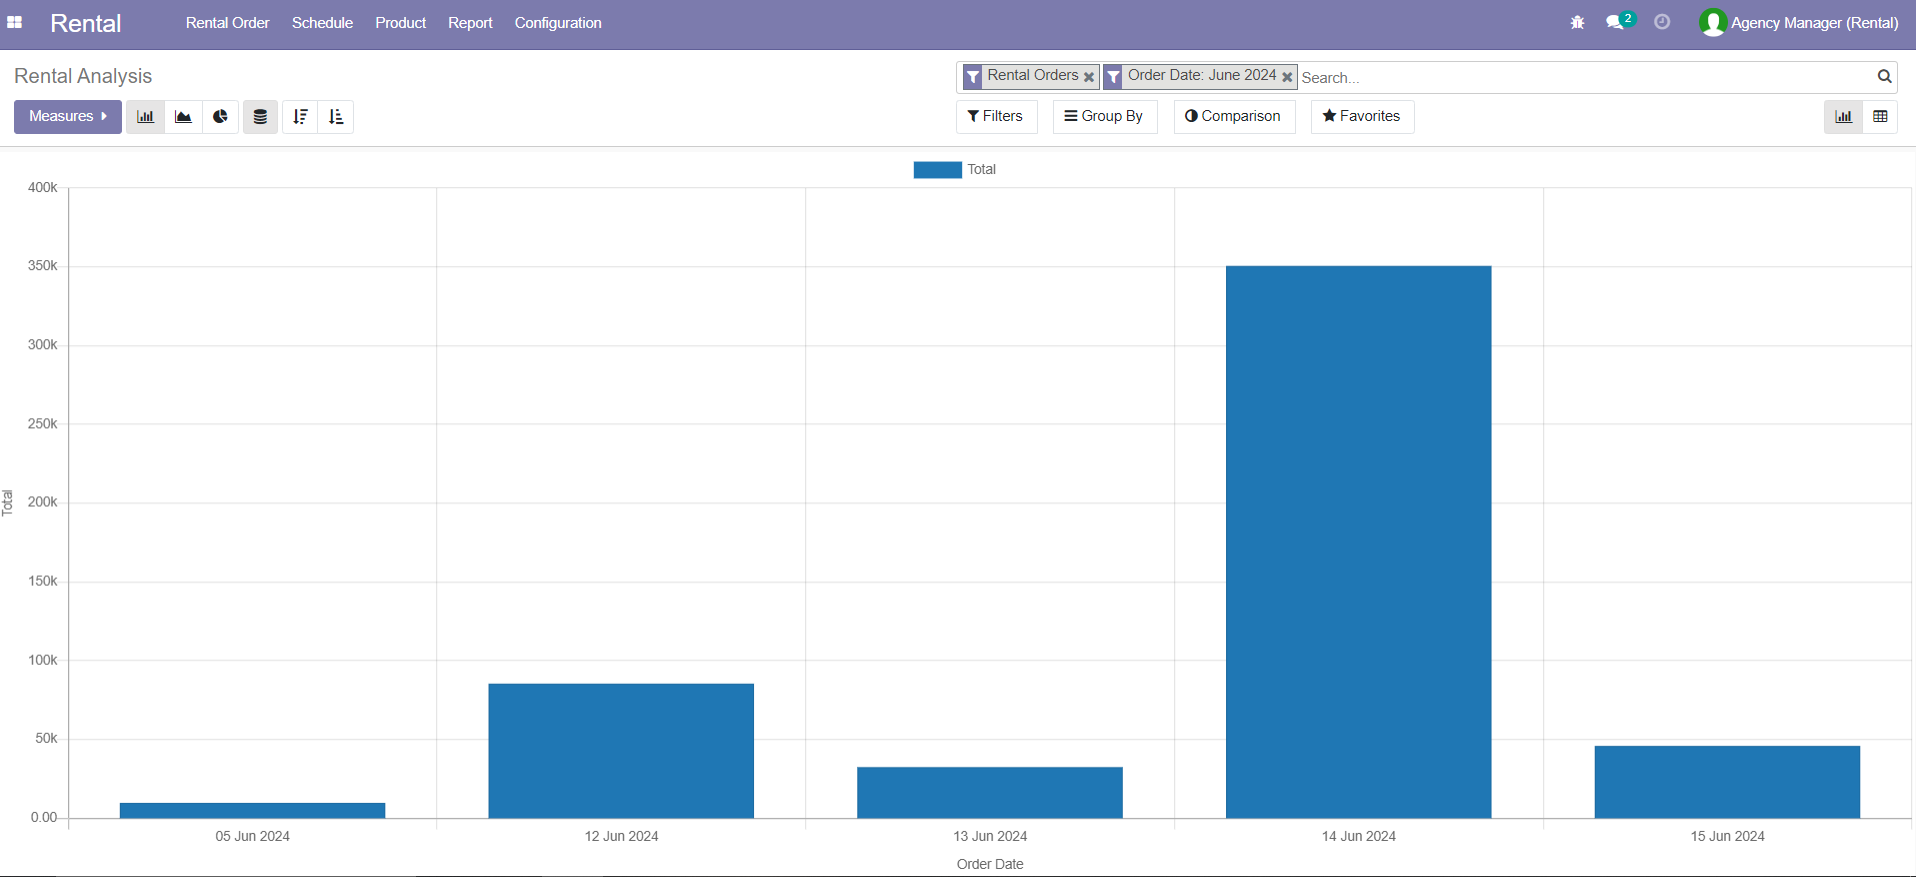
\includegraphics[width=0.8\textwidth]{sprint3/reportbarchart.png} % replace with your image path
    \caption{Screenshot of Rental Order Report - Bar Chart View}
    \label{fig:bar_chart_view}
\end{figure}

\subsection{Pie Chart View}
Figure \ref{fig:pie_chart_view} presents the rental order report in a pie chart format. This view is useful for understanding the distribution of rental orders across different categories.

\begin{figure}[h]
    \centering
    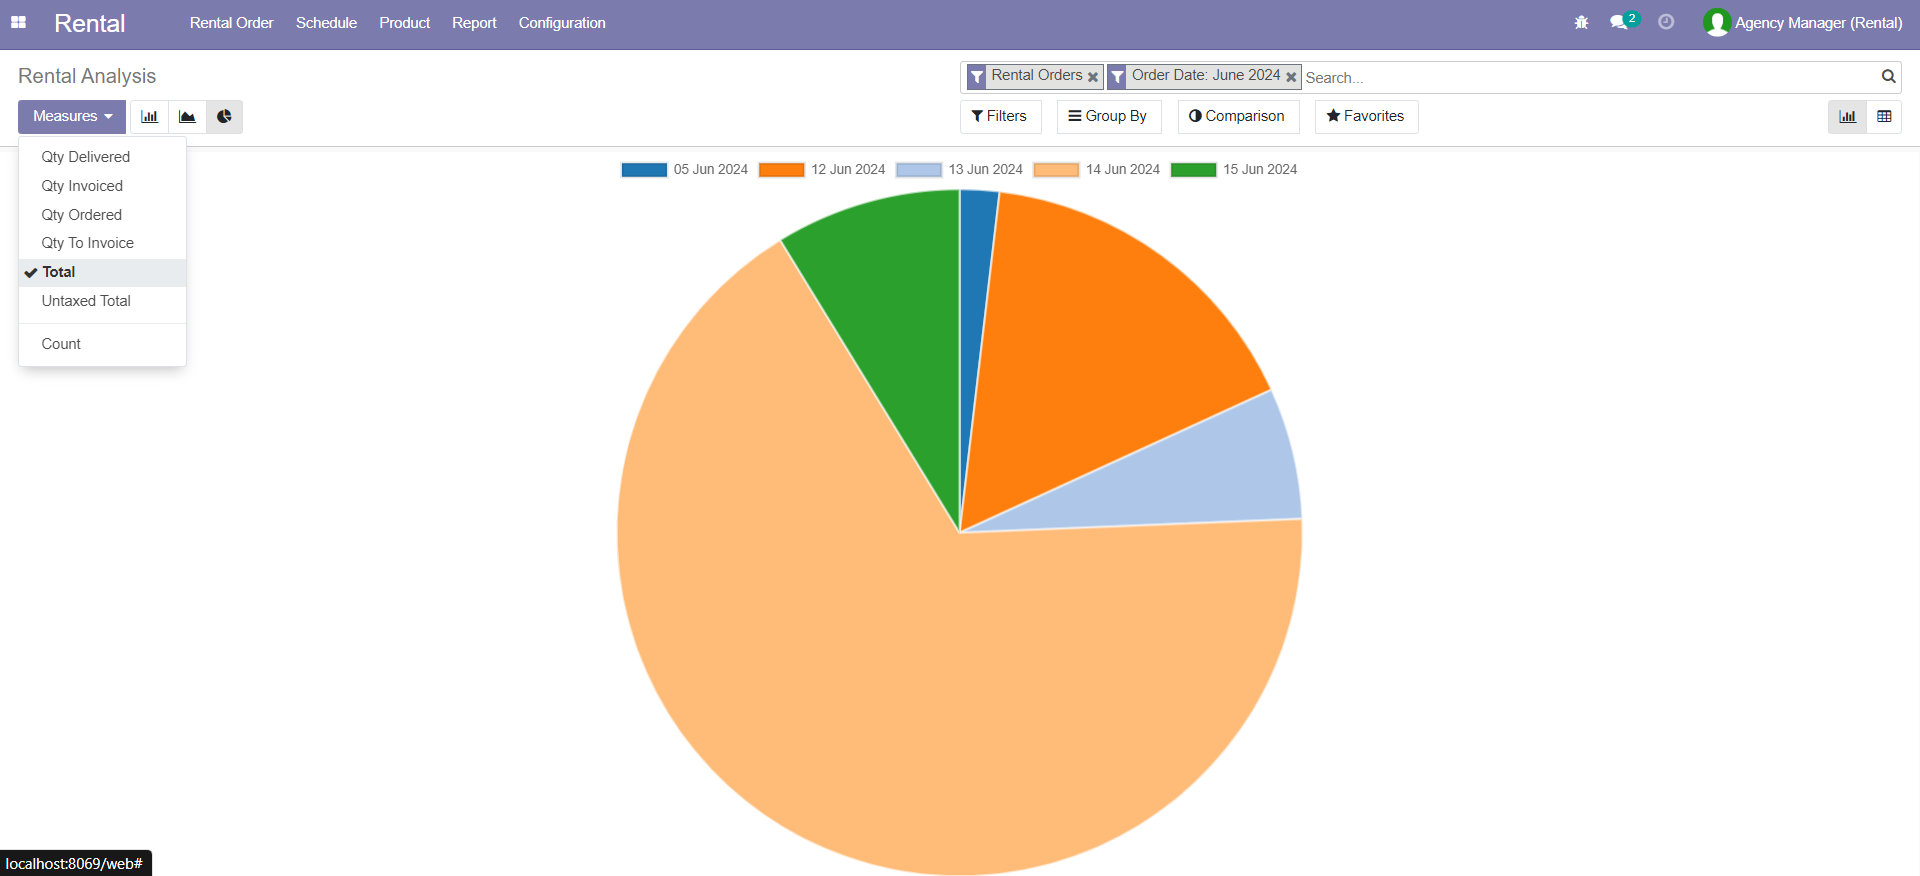
\includegraphics[width=0.8\textwidth]{sprint3/reportpiechart.png} % replace with your image path
    \caption{Screenshot of Rental Order Report - Pie Chart View}
    \label{fig:pie_chart_view}
\end{figure}

\subsection{Line Chart View}
Figure \ref{fig:line_chart_view} displays the rental order report in a line chart format. This view is ideal for observing trends in rental orders over time.

\begin{figure}[h]
    \centering
    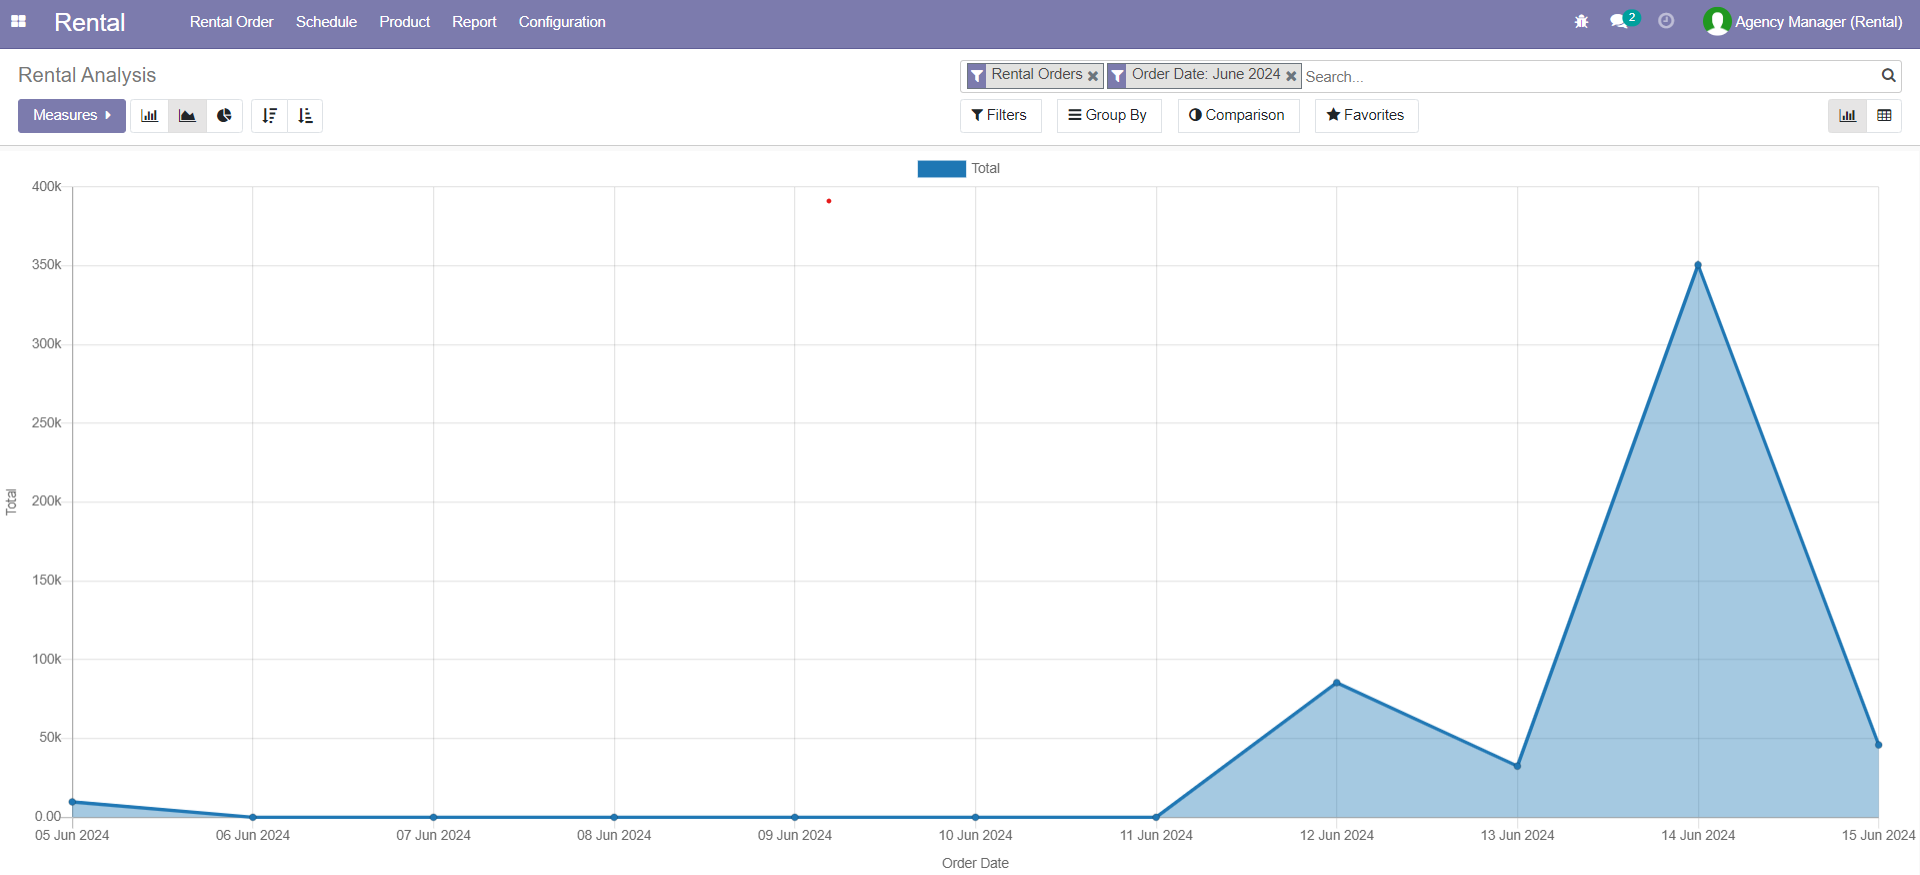
\includegraphics[width=0.8\textwidth]{sprint3/reportlinechart.png} % replace with your image path
    \caption{Screenshot of Rental Order Report - Line Chart View}
    \label{fig:line_chart_view}
\end{figure}

\subsection{Pivot Chart View}
Figure \ref{fig:pivot_chart_view} illustrates the rental order report in a pivot chart format. This view allows for dynamic data analysis and in-depth exploration of rental order details.

\begin{figure}[h]
    \centering
    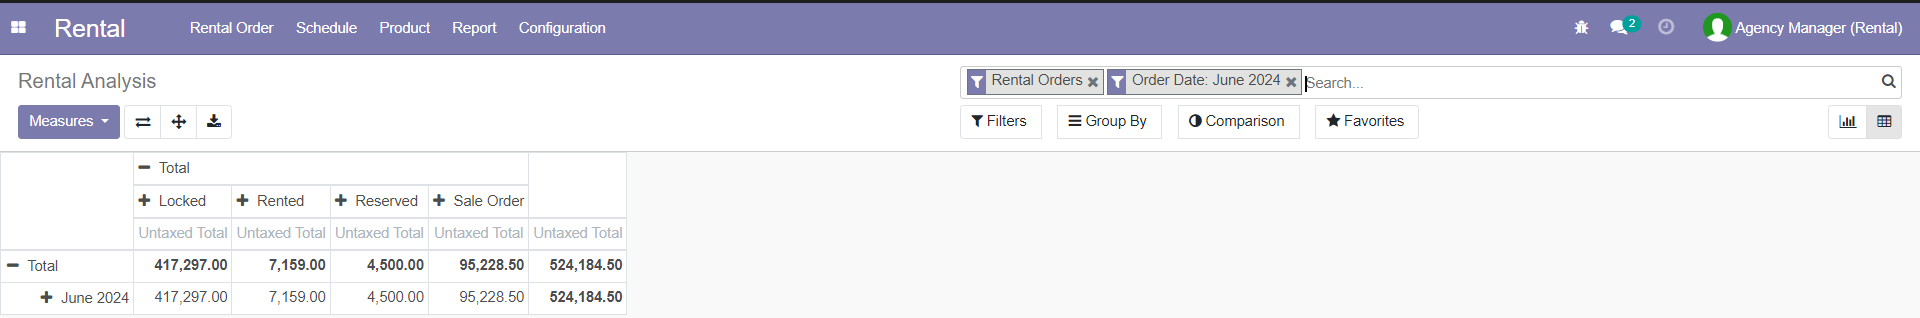
\includegraphics[width=0.\textwidth]{sprint3/reportpivot.png} % replace with your image path
    \caption{Screenshot of Rental Order Report - Pivot Chart View}
    \label{fig:pivot_chart_view}
\end{figure}



\section*{Conclusion}
\addcontentsline{toc}{section}{Conclusion}
In Sprint 3, we enhanced the rental order reporting in Odoo ERP, enabling administrators to generate and analyze reports in various chart formats with dynamic filters. In the next sprint, we will focus on integrating these reporting capabilities with the billing and invoicing module, allowing administrators to manage the system effectively.
.
